\documentclass{standalone}
\usepackage{tikz}
\usetikzlibrary{patterns, positioning}

\begin{document}
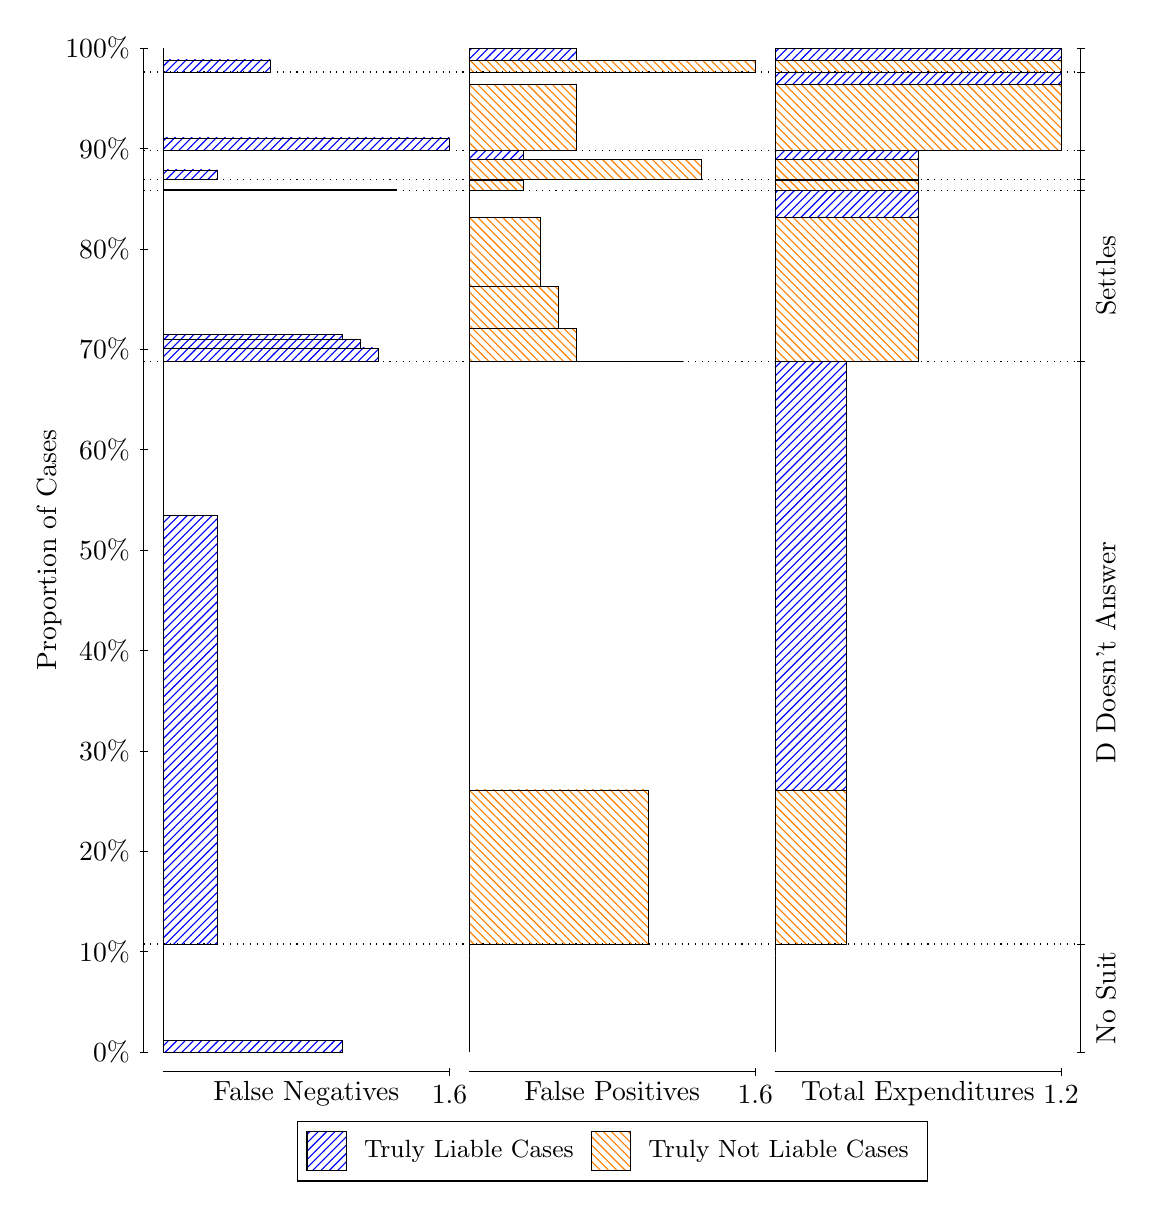
\begin{tikzpicture}
\draw[black, very thin] (1.5,1.75) -- (1.5,14.5);
\node[rotate=90, anchor=center] at (0.3, 8.125) {Proportion of Cases};
\draw[black, very thin] (1.45,1.75) -- (1.55,1.75);
\node[anchor=east] at (1.45, 1.75) {0\%};
\draw[black, very thin] (1.45,3.025) -- (1.55,3.025);
\node[anchor=east] at (1.45, 3.025) {10\%};
\draw[black, very thin] (1.45,4.3) -- (1.55,4.3);
\node[anchor=east] at (1.45, 4.3) {20\%};
\draw[black, very thin] (1.45,5.575) -- (1.55,5.575);
\node[anchor=east] at (1.45, 5.575) {30\%};
\draw[black, very thin] (1.45,6.85) -- (1.55,6.85);
\node[anchor=east] at (1.45, 6.85) {40\%};
\draw[black, very thin] (1.45,8.125) -- (1.55,8.125);
\node[anchor=east] at (1.45, 8.125) {50\%};
\draw[black, very thin] (1.45,9.4) -- (1.55,9.4);
\node[anchor=east] at (1.45, 9.4) {60\%};
\draw[black, very thin] (1.45,10.675) -- (1.55,10.675);
\node[anchor=east] at (1.45, 10.675) {70\%};
\draw[black, very thin] (1.45,11.95) -- (1.55,11.95);
\node[anchor=east] at (1.45, 11.95) {80\%};
\draw[black, very thin] (1.45,13.225) -- (1.55,13.225);
\node[anchor=east] at (1.45, 13.225) {90\%};
\draw[black, very thin] (1.45,14.5) -- (1.55,14.5);
\node[anchor=east] at (1.45, 14.5) {100\%};

\draw[black, very thin] (13.4,1.75) -- (13.4,14.5);
\draw[black, very thin] (13.35,1.75) -- (13.45,1.75);
\node[anchor=west] at (13.35, 1.75) {};
\draw[black, very thin] (13.35,3.1214) -- (13.45,3.1214);
\node[anchor=west] at (13.35, 3.1214) {};
\draw[black, very thin] (13.35,10.52) -- (13.45,10.52);
\node[anchor=west] at (13.35, 10.52) {};
\draw[black, very thin] (13.35,12.696) -- (13.45,12.696);
\node[anchor=west] at (13.35, 12.696) {};
\draw[black, very thin] (13.35,12.831) -- (13.45,12.831);
\node[anchor=west] at (13.35, 12.831) {};
\draw[black, very thin] (13.35,13.203) -- (13.45,13.203);
\node[anchor=west] at (13.35, 13.203) {};
\draw[black, very thin] (13.35,14.195) -- (13.45,14.195);
\node[anchor=west] at (13.35, 14.195) {};
\draw[black, very thin] (13.35,14.5) -- (13.45,14.5);
\node[anchor=west] at (13.35, 14.5) {};

\draw[black, very thin, pattern color=blue, pattern=north east lines] (1.75,1.75) rectangle (4.0208,1.8943);
\draw[black, very thin, pattern color=orange, pattern=north west lines] (1.75,1.8943) rectangle (1.75,3.1214);
\draw[black, very thin, pattern color=blue, pattern=north east lines] (1.75,3.1214) rectangle (2.4312,8.5642);
\draw[black, very thin, pattern color=orange, pattern=north west lines] (1.75,8.5642) rectangle (1.75,10.52);
\draw[black, very thin, pattern color=blue, pattern=north east lines] (1.75,10.52) rectangle (4.475,10.692);
\draw[black, very thin, pattern color=blue, pattern=north east lines] (1.75,10.692) rectangle (4.2479,10.795);
\draw[black, very thin, pattern color=blue, pattern=north east lines] (1.75,10.795) rectangle (4.0208,10.867);
\draw[black, very thin, pattern color=blue, pattern=north east lines] (1.75,10.867) rectangle (3.7937,10.867);
\draw[black, very thin, pattern color=blue, pattern=north east lines] (1.75,10.867) rectangle (3.7937,10.867);
\draw[black, very thin, pattern color=blue, pattern=north east lines] (1.75,10.867) rectangle (3.5667,10.867);
\draw[black, very thin, pattern color=blue, pattern=north east lines] (1.75,10.867) rectangle (3.3396,10.867);
\draw[black, very thin, pattern color=blue, pattern=north east lines] (1.75,10.867) rectangle (3.1125,10.867);
\draw[black, very thin, pattern color=blue, pattern=north east lines] (1.75,10.867) rectangle (2.8854,10.867);
\draw[black, very thin, pattern color=blue, pattern=north east lines] (1.75,10.867) rectangle (2.6583,10.867);
\draw[black, very thin, pattern color=orange, pattern=north west lines] (1.75,10.867) rectangle (1.75,12.696);
\draw[black, very thin, pattern color=blue, pattern=north east lines] (1.75,12.696) rectangle (4.7021,12.707);
\draw[black, very thin, pattern color=orange, pattern=north west lines] (1.75,12.707) rectangle (1.75,12.831);
\draw[black, very thin, pattern color=blue, pattern=north east lines] (1.75,12.831) rectangle (2.4312,12.953);
\draw[black, very thin, pattern color=orange, pattern=north west lines] (1.75,12.953) rectangle (1.75,13.203);
\draw[black, very thin, pattern color=blue, pattern=north east lines] (1.75,13.203) rectangle (5.3833,13.358);
\draw[black, very thin, pattern color=orange, pattern=north west lines] (1.75,13.358) rectangle (1.75,14.195);
\draw[black, very thin, pattern color=blue, pattern=north east lines] (1.75,14.195) rectangle (3.1125,14.349);
\draw[black, very thin, pattern color=orange, pattern=north west lines] (1.75,14.349) rectangle (1.75,14.5);
\draw[black, very thin, pattern color=orange, pattern=north west lines] (5.6333,1.75) rectangle (5.6333,2.9771);
\draw[black, very thin, pattern color=blue, pattern=north east lines] (5.6333,2.9771) rectangle (5.6333,3.1214);
\draw[black, very thin, pattern color=orange, pattern=north west lines] (5.6333,3.1214) rectangle (7.9042,5.0776);
\draw[black, very thin, pattern color=blue, pattern=north east lines] (5.6333,5.0776) rectangle (5.6333,10.52);
\draw[black, very thin, pattern color=orange, pattern=north west lines] (5.6333,10.52) rectangle (8.3583,10.52);
\draw[black, very thin, pattern color=orange, pattern=north west lines] (5.6333,10.52) rectangle (8.1313,10.52);
\draw[black, very thin, pattern color=orange, pattern=north west lines] (5.6333,10.52) rectangle (7.9042,10.52);
\draw[black, very thin, pattern color=orange, pattern=north west lines] (5.6333,10.52) rectangle (7.6771,10.52);
\draw[black, very thin, pattern color=orange, pattern=north west lines] (5.6333,10.52) rectangle (7.45,10.52);
\draw[black, very thin, pattern color=orange, pattern=north west lines] (5.6333,10.52) rectangle (7.2229,10.52);
\draw[black, very thin, pattern color=orange, pattern=north west lines] (5.6333,10.52) rectangle (6.9958,10.937);
\draw[black, very thin, pattern color=orange, pattern=north west lines] (5.6333,10.937) rectangle (6.7687,11.469);
\draw[black, very thin, pattern color=orange, pattern=north west lines] (5.6333,11.469) rectangle (6.5417,12.349);
\draw[black, very thin, pattern color=blue, pattern=north east lines] (5.6333,12.349) rectangle (6.0875,12.349);
\draw[black, very thin, pattern color=blue, pattern=north east lines] (5.6333,12.349) rectangle (5.8604,12.349);
\draw[black, very thin, pattern color=blue, pattern=north east lines] (5.6333,12.349) rectangle (5.6333,12.696);
\draw[black, very thin, pattern color=orange, pattern=north west lines] (5.6333,12.696) rectangle (6.3146,12.821);
\draw[black, very thin, pattern color=blue, pattern=north east lines] (5.6333,12.821) rectangle (5.6333,12.831);
\draw[black, very thin, pattern color=orange, pattern=north west lines] (5.6333,12.831) rectangle (8.5854,13.081);
\draw[black, very thin, pattern color=blue, pattern=north east lines] (5.6333,13.081) rectangle (6.3146,13.203);
\draw[black, very thin, pattern color=orange, pattern=north west lines] (5.6333,13.203) rectangle (6.9958,14.04);
\draw[black, very thin, pattern color=blue, pattern=north east lines] (5.6333,14.04) rectangle (5.6333,14.195);
\draw[black, very thin, pattern color=orange, pattern=north west lines] (5.6333,14.195) rectangle (9.2667,14.346);
\draw[black, very thin, pattern color=blue, pattern=north east lines] (5.6333,14.346) rectangle (6.9958,14.5);
\draw[black, very thin, pattern color=orange, pattern=north west lines] (9.5167,1.75) rectangle (9.5167,2.9771);
\draw[black, very thin, pattern color=blue, pattern=north east lines] (9.5167,2.9771) rectangle (9.5167,3.1214);
\draw[black, very thin, pattern color=orange, pattern=north west lines] (9.5167,3.1214) rectangle (10.425,5.0776);
\draw[black, very thin, pattern color=blue, pattern=north east lines] (9.5167,5.0776) rectangle (10.425,10.52);
\draw[black, very thin, pattern color=orange, pattern=north west lines] (9.5167,10.52) rectangle (11.333,10.52);
\draw[black, very thin, pattern color=blue, pattern=north east lines] (9.5167,10.52) rectangle (11.333,10.52);
\draw[black, very thin, pattern color=orange, pattern=north west lines] (9.5167,10.52) rectangle (11.333,12.349);
\draw[black, very thin, pattern color=blue, pattern=north east lines] (9.5167,12.349) rectangle (11.333,12.696);
\draw[black, very thin, pattern color=orange, pattern=north west lines] (9.5167,12.696) rectangle (11.333,12.696);
\draw[black, very thin, pattern color=blue, pattern=north east lines] (9.5167,12.696) rectangle (11.333,12.696);
\draw[black, very thin, pattern color=orange, pattern=north west lines] (9.5167,12.696) rectangle (11.333,12.821);
\draw[black, very thin, pattern color=blue, pattern=north east lines] (9.5167,12.821) rectangle (11.333,12.831);
\draw[black, very thin, pattern color=orange, pattern=north west lines] (9.5167,12.831) rectangle (11.333,13.081);
\draw[black, very thin, pattern color=blue, pattern=north east lines] (9.5167,13.081) rectangle (11.333,13.203);
\draw[black, very thin, pattern color=orange, pattern=north west lines] (9.5167,13.203) rectangle (13.15,14.04);
\draw[black, very thin, pattern color=blue, pattern=north east lines] (9.5167,14.04) rectangle (13.15,14.195);
\draw[black, very thin, pattern color=orange, pattern=north west lines] (9.5167,14.195) rectangle (13.15,14.346);
\draw[black, very thin, pattern color=blue, pattern=north east lines] (9.5167,14.346) rectangle (13.15,14.5);
\draw[black, dotted] (1.5,3.1214) -- (13.4,3.1214);
\draw[black, dotted] (1.5,10.52) -- (13.4,10.52);
\draw[black, dotted] (1.5,12.696) -- (13.4,12.696);
\draw[black, dotted] (1.5,12.831) -- (13.4,12.831);
\draw[black, dotted] (1.5,13.203) -- (13.4,13.203);
\draw[black, dotted] (1.5,14.195) -- (13.4,14.195);
\draw[black, very thin] (1.75,1.5) -- (5.3833,1.5);
\node[anchor=north] at (3.5667, 1.5) {False Negatives};
\draw[black, very thin] (5.3833,1.45) -- (5.3833,1.55);
\node[anchor=north] at (5.3833, 1.45) {1.6};

\draw[black, very thin] (5.6333,1.5) -- (9.2667,1.5);
\node[anchor=north] at (7.45, 1.5) {False Positives};
\draw[black, very thin] (9.2667,1.45) -- (9.2667,1.55);
\node[anchor=north] at (9.2667, 1.45) {1.6};

\draw[black, very thin] (9.5167,1.5) -- (13.15,1.5);
\node[anchor=north] at (11.333, 1.5) {Total Expenditures};
\draw[black, very thin] (13.15,1.45) -- (13.15,1.55);
\node[anchor=north] at (13.15, 1.45) {1.2};

\node[black, centered, rotate=90] at (13.72, 2.4357) {No Suit};
\node[black, centered, rotate=90] at (13.72, 6.8209) {D Doesn't Answer};
\node[black, centered, rotate=90] at (13.72, 11.608) {Settles};





\draw (7.449999999999999,1.5) node[draw=none] (baseCoordinate) {};
\begin{scope}[align=center]
        \matrix[scale=0.5, draw=black, below=0.5cm of baseCoordinate, nodes={draw}, column sep=0.1cm]{
            \node[rectangle, draw, minimum width=0.5cm, minimum height=0.5cm, pattern=north east lines, pattern color=blue] {}; &
            \node[draw=none, font=\small] (B) {Truly Liable Cases}; &
            \node[rectangle, draw, minimum width=0.5cm, minimum height=0.5cm, pattern=north west lines, pattern color=orange] {}; &
            \node[draw=none, font=\small] (B) {Truly Not Liable Cases}; \\
            };
\end{scope}

\end{tikzpicture}
\end{document}